\chapter{Arkitektur}
I dette afsnit vil der blive beskrevet den overordnede arkitektur for Rambøll Tilsyn.

På Figur \ref{fig:Domain} ses domæne modellen for Rambøll Tilsyn. Her ses, hvilke dele systemet indeholder og hvilken relation de har til hinanden.
For den fulde arkitektur henvises til Arkitektur og Design dokumentationens afsnit \ref{Design-sec:Arkitektur}

\begin{figure}[H] % (alternativt [H])
	\centering
	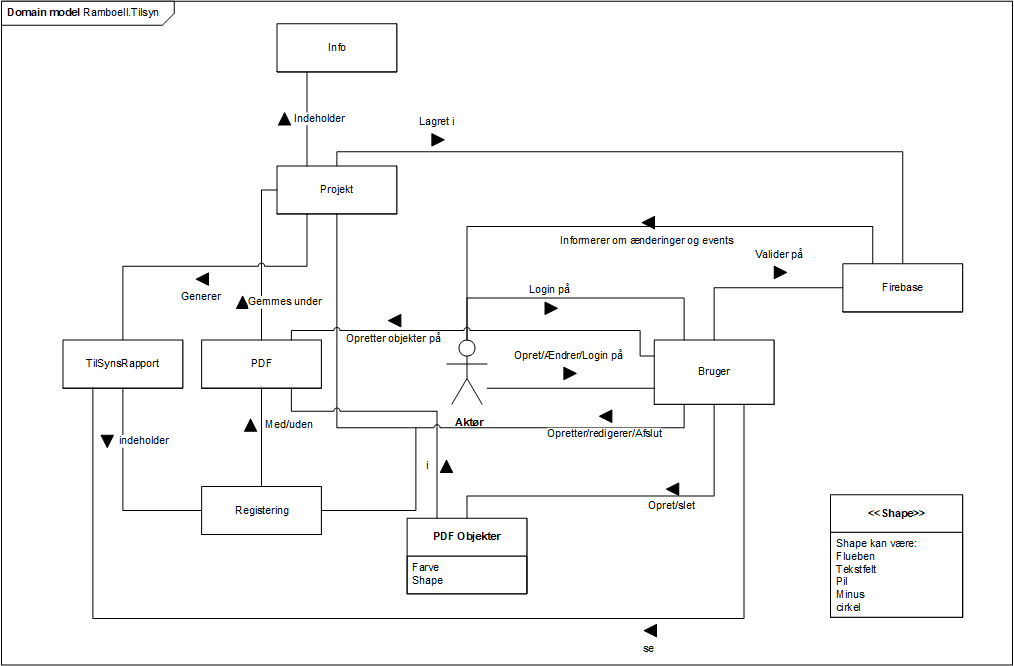
\includegraphics[height=13cm, width=17cm]{Arkitektur/Domainmodel}
	\caption{Domænemodel for Rambøll Tilsyn.}
	\label{fig:Domain}
\end{figure}

\clearpage


\begin{figure}[H] % (alternativt [H])
	\centering
	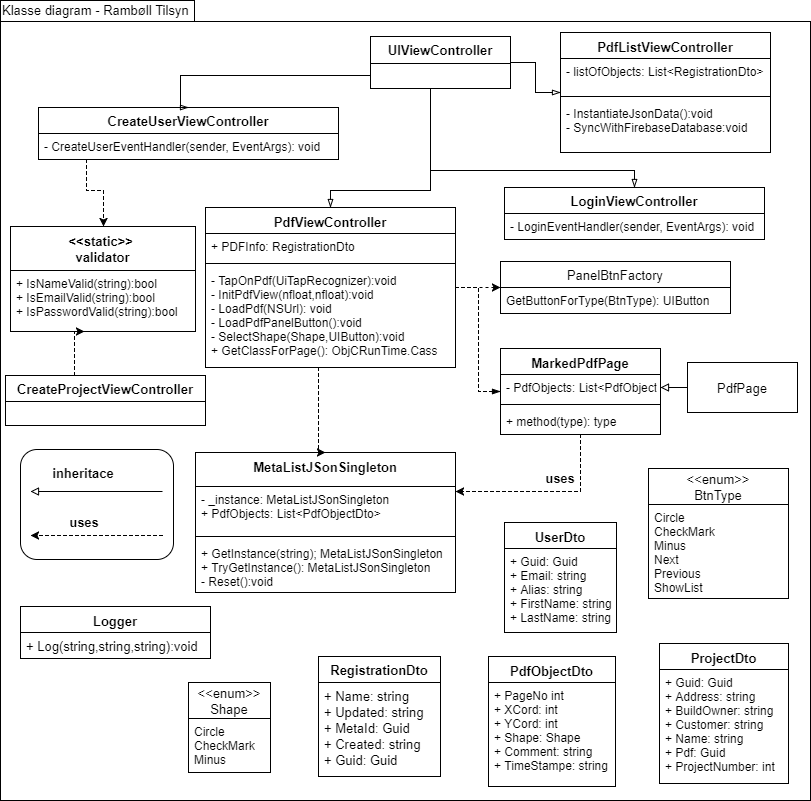
\includegraphics[height=13cm, width=17cm]{Arkitektur/KlasseDiagram}
	\caption{Klassediagram for Rambøll Tilsyn.}
	\label{fig:KlasseDiagram}
\end{figure}

